\documentclass{article}
\usepackage[utf8]{inputenc}
\usepackage{graphicx}
\usepackage{geometry}
\geometry{margin=1in}

\title{Database Design: Solved Problems}
\author{Adoración de Miguel Castaño}
\date{September 2000}

\begin{document}

\maketitle

\section{Conceptual Design: E-R MODEL}

\subsection{Introduction}

\subsubsection{Methodological guides to approach the resolution of problems}

The elaboration of an E-R scheme that captures the semantics of a certain Universe of Discourse is a creative process for which there is no defined procedure.  However, it is possible to follow a series of recommendations or heuristics that help us in the design. These recommendations are not rules that always work but in some cases are appropriate and in others not.

\subsubsection{
Some Heuristics for the Identification of the Different Constructs}

In the first proposal of the E-R Model (Chen, 1976), only three classes of objects are distinguished: entities, attributes, and relationships. The model that will be used in the conceptual modeling phase in the exercises of this book is the extended E-R model that adds to the basic model a set of constructs that help to collect more semantics of the universe of discourse (minimum and maximum cardinalities in relationships, generalizations, dependence in existence and identification, etc.).  It is not really a single model but a family of models, since each author specializes it and adds different constructs to it.  The complete description of this model is found in De Miguel et al. (1999). In this section, the constructs that make up the extended E-R model will be briefly explained in order to facilitate the understanding of the problems.

Entities are the main objects about which information should be collected and generally denote people, places, things, or events of interest.  Entities will usually appear in the statement as nouns.  Each of the possible occurrences (each specific person, place, thing, or event) of the entity is called an instance.

Attributes are used to detail entities by assigning them descriptive properties such as name, color, and weight.  There are two types of attributes: identifiers and descriptors.  The former are used to uniquely distinguish each of the occurrences of an entity (distinguishing between Primary Identifiers and Alternative Identifiers), while the descriptors are used to describe an entity occurrence.  It is not only possible to specify attributes in entities but also in relationships (in this case it only makes sense to talk about descriptive attributes and not identifiers).  Attributes will also be reflected in the statement, generally, as nouns.

In relation to attributes, there is also the concept of a domain (a set of values over which the attribute is defined).  Although they can be represented explicitly in the E-R schemes (as shown in the following section where the notations are reflected), in the problems of this book it will be considered that the domain takes the same name as the attribute.  For example, the \texttt{EMPLOYEE} entity may have the \textit{"Marital Status"} attribute defined on the \textit{"Marital Statuses"} domain (composed of the values Single, Married, Widowed, Divorced) and whose two possible representations in the E-R scheme are shown in figure 1.1.

\begin{figure}
    \centering
    % Placeholder for Figure 1.1
    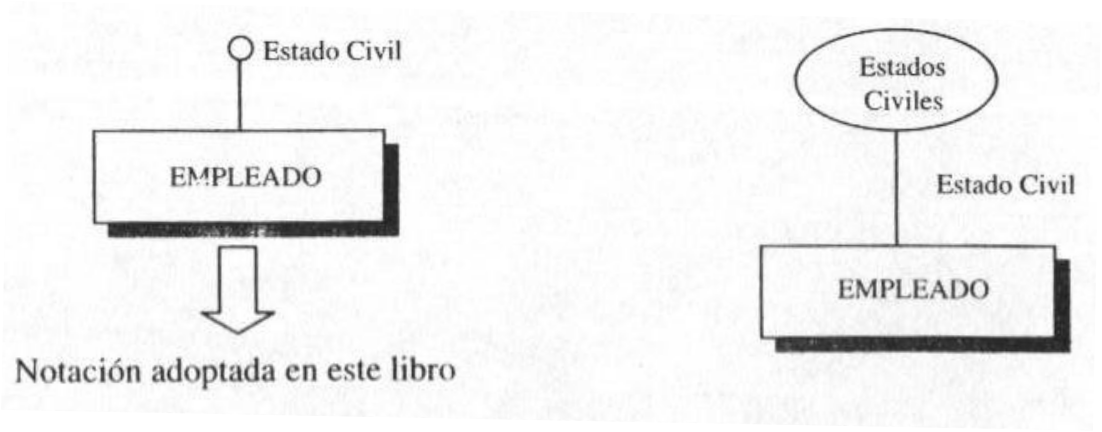
\includegraphics[width=0.8\textwidth]{figures/fig1}
    \caption{Representation of domains. The image shows two ways to represent the relationship between an \texttt{EMPLOYEE} entity and their \textit{Marital Status}. The left diagram shows \textit{"Estado Civil"} (Marital Status) as an attribute of \texttt{EMPLOYEE}. The right diagram shows \textit{"Estados Civiles"} (Marital Statuses) as a separate entity connected to \texttt{EMPLOYEE} by a relationship labeled \textit{"Estado Civil"}.}
    \label{fig:fig1.1}
\end{figure}

It is also possible to collect other semantic restrictions on the attributes apart from the already mentioned ones of Primary and Alternative Identifier attributes.  Thus, we speak of mandatory/optional attributes (if an attribute must take a value or not), single-valued/multi-valued attributes (if an attribute takes a single value or several), derived attributes (if its value is obtained from other elements of the E-R scheme), and simple/composite attributes (depending on whether an attribute is an aggregate of other attributes or not).  In turn, these restrictions can be combined with each other (there can be in an E-R scheme optional simple multi-valued attributes, optional composite single-valued attributes, mandatory multi-valued attributes, composite multi-valued attributes, etc.).

Entities can be classified by the strength of their identifying attributes, that is, by their dependence or non-dependence on other entities.  Strong entities have their own existence, that is, they have internal identifiers that uniquely determine the existence of their occurrences.  Weak entities can be so for two reasons: either because their existence in the DB depends on a strong entity, or because they require for their identification the identifying attributes (sometimes called external attributes) of another entity, for example, they do not have internal identifying attributes that allow the identification of each of their occurrences and require the presence of external attributes.  In the first of the cases, we speak of Dependence in Existence and in the second of Dependence in Identification.

Finally, relationships represent real-world associations between one or more entities.  Relationships are characterized by their name, the degree (number of entities participating in the relationship), the type of correspondence (maximum number of instances of one entity associated with a combination of instances of the other entities in the relationship, which can be 1 or N).  Thus, in the example in figure 1.2, it is observed that the correspondence type of the Participate relationship is 1:N, that is, an employee participates in at most one project and in one project at most N employees participate.  As with entities, an instance of the relationship is each combination of instances of the interrelated entities that constitute an occurrence in the relationship.

A construct that extends the semantics collected in a relationship is the cardinality constraint.  The maximum and minimum cardinalities of the entities participating in a relationship are defined as the maximum and minimum number of instances of an entity that can be related to a single instance of the other, or other entities participating in the relationship.  Graphically, cardinality constraints are represented by a label, (0,1), (1,1), (0,N), or (1,N), located on the line connecting the entity with the diamond that represents the type of relationship (see figure 1.2).

\begin{figure}
    \centering
    % Placeholder for Figure 1.2
    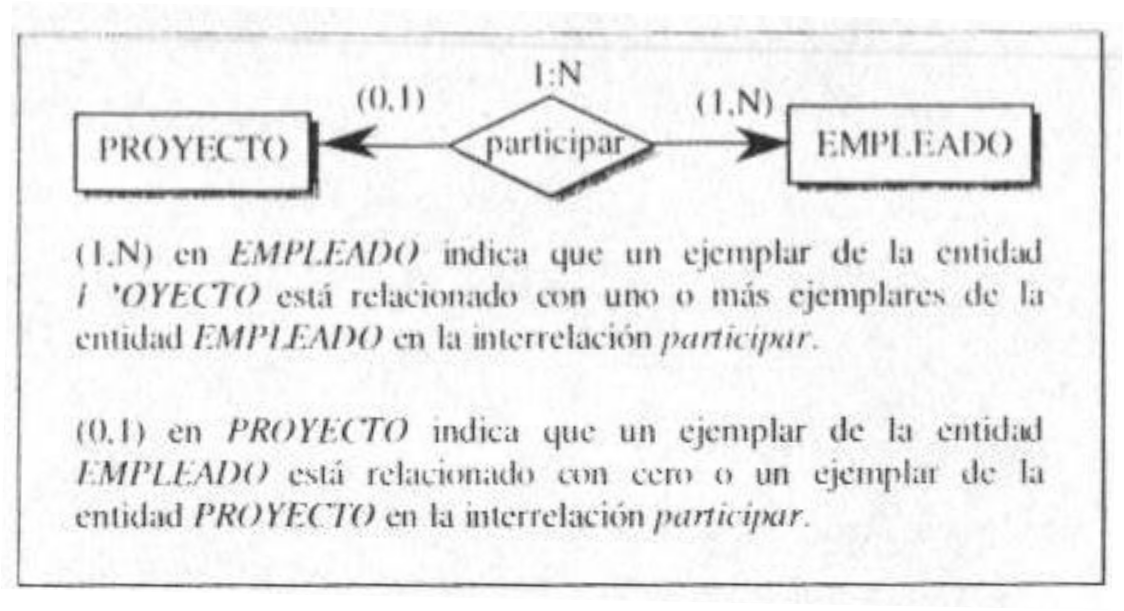
\includegraphics[width=0.8\textwidth]{figures/fig2}
    \caption{Example of minimum and maximum cardinalities. The diagram shows a "participar" (\textit{participate}) relationship between \texttt{PROJECT} and \texttt{EMPLOYEE}. The notation (1,N) on the \texttt{EMPLOYEE} side indicates that a \texttt{PROJECT} instance is related to one or more \texttt{EMPLOYEE} instances. The notation (0,1) on the \texttt{PROJECT} side indicates that an \texttt{EMPLOYEE} instance is related to zero or one \texttt{PROJECT} instances.}
    \label{fig:fig1.2}
\end{figure}

In the statements, the appearance of verbs may indicate, in some cases, the existence of a relationship in the E-R scheme.

As for generalizations, they provide us with an abstraction mechanism that allows specializing an entity (which will be called a supertype) into subtypes, or what is the same, generalizing the subtypes into the supertype.  In this way we see a set of occurrences of one entity as occurrences of another entity (as also happens in the "is\_a" hierarchies of semantic networks).  For example, a "Person" is an "Animal" and a "Reptile" is an "Animal"; in this case, "Animal" can be considered the supertype and "Person" and "Reptile" are subtypes of "Animal".  The occurrences or instances of "Person" are also of "Animal" and the same happens with those of "Reptile".

We will be able to identify generalizations if we find a series of attributes common to a set of entities.  This situation occurs frequently if a view integration process is being carried out, De Miguel et al. (1999).  These common attributes will describe the supertype and the particular attributes will remain in the subtypes.  It may happen that the subtypes do not have their own attributes; in that case, subtypes will only exist (even if to better capture the semantics, they can be reflected) if they are going to participate in relationships (apart from the relationships in which the supertype participates).

For example, suppose the following entities identified in a universe of discourse of a company: EMPLOYEE (with identifier "Emp-No" and the descriptors "Emp-Name", "Family-Address", "Birth-Date", "Job-Description", "Salary", "Experience"), ENGINEER (with identifier "Emp-No" and descriptors "Emp-Name", "Family-Address", "Specialty"), SECRETARY (with identifier "Emp-No" and descriptors "Emp-Name", "Birth-Date", "Salary", "Typing-Speed"), TECHNICIAN (with identifier "Emp-No" and descriptors "Emp-Name", "Experience", "Years-of-Experience").  We identify that EMPLOYEE is a generalization of ENGINEER, SECRETARY, and TECHNICIAN.  Then we redistribute the attributes among the entities.  We place the identifier "Emp-No" and the generic descriptors "Emp-Name", "Family-Address", "Birth-Date", "Job-Description", and "Salary" in the supertype entity EMPLOYEE, we put the specific descriptor "Specialty" in the ENGINEER entity; we put the specific descriptor "Typing-Speed" in the SECRETARY entity and, finally, we put the specific descriptors "Experience" and "Years-Experience" in the TECHNICIAN entity.  Figure 1.3 shows the resulting E-R scheme.

\begin{figure}
    \centering
    % Placeholder for Figure 1.3
    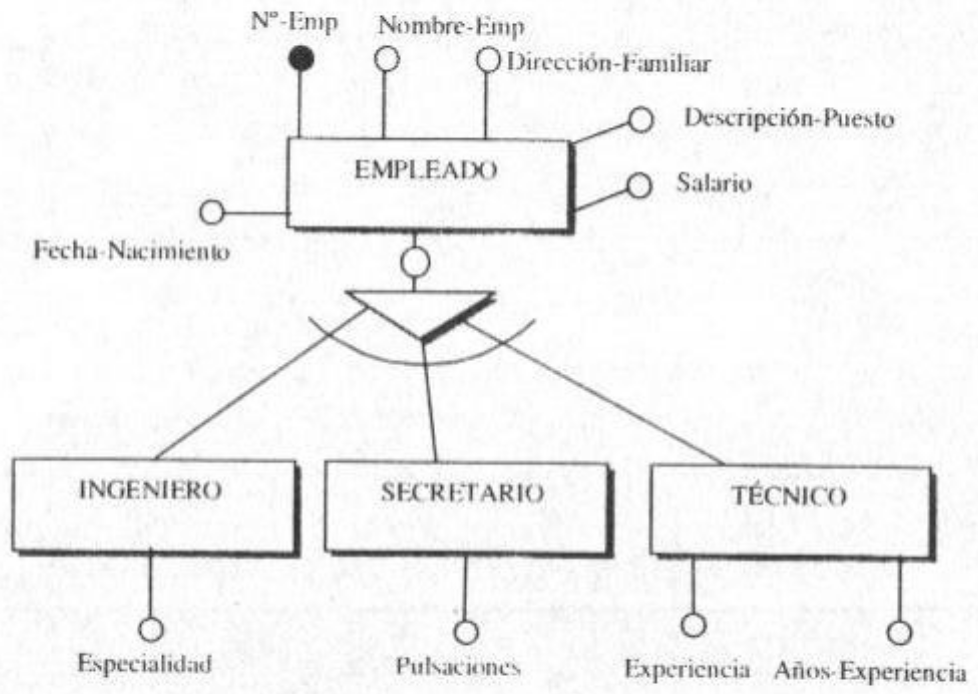
\includegraphics[width=0.8\textwidth]{figures/fig3}
    \caption{Example of generalization. The diagram shows a generalization hierarchy where EMPLOYEE is the supertype and ENGINEER, SECRETARY, and TECHNICIAN are subtypes. Attributes common to all employees are attached to the EMPLOYEE entity, while attributes specific to each job role are attached to their respective subtype entities.}
    \label{fig:fig1.3}
\end{figure}

There are other semantic restrictions related to generalizations such as totality/partiality and exclusivity/overlapping.  If the occurrences of the subtypes of a generalization cover the supertype (that is, there are no occurrences in the supertype that do not belong to any of the subtypes) then it is a total generalization and otherwise partial.  On the other hand, if there can be occurrences that belong to more than one of the subtypes then it is a generalization with overlapping; in case the subtypes are disjoint, we speak of exclusive generalizations.  The example in Figure 1.3 shows a total generalization, that is, there are no EMPLOYEES who are neither ENGINEERS, nor SECRETARIES, nor TECHNICIANS; in addition, it is an exclusive generalization, that is, an EMPLOYEE is either an ENGINEER, a SECRETARY, or a TECHNICIAN, but cannot be several things at the same time.

\subsection{
Some Heuristics for Choosing between Various Constructs
}

Although it is simple to define the constructs of entity, attribute, and relationship, it is not so simple to distinguish their role in DB modeling.  What makes a concept an attribute, an entity, or a relationship?; in this case, one can only resort to a series of heuristics that help us decide between one of the constructs that can reflect the semantics of a certain concept.  Some of them are described below.

\subsubsection{Entities vs. attributes}

Attributes do not have existence by themselves but make sense as they belong to a certain entity or relationship.  An entity must be characterized by something more than its Primary Identifier.  If there is descriptive information about a concept or object, then it should be classified as an entity.  If only one identifier is needed for an object, the object should be classified as an attribute.  Thus, \textbf{entities have descriptive information and attributes do not}.

For example, in the assumption "Warehouses are located in Cities".  If there is some descriptive information about the State and Population of the Cities, then City should be classified as an entity.  If only the "City Name" attribute is needed to identify a city, then it should be classified as an attribute.  On the other hand, it could happen that even having a concept for which there is only one Primary Identifier, it is related to more than one entity.  In that case, it could appear as an entity in the E-R scheme.  In the previous example, if there was another assumption "suppliers are assigned several cities", then City could be left as an entity related to the Warehouse and Supplier entities or left as attributes in both entities.

\subsubsection{Entities vs. multi-valued attributes}

In this aspect there are discrepancies.  There are proposals that prefer to incorporate in the E-R schemes a multi-valued attribute as an entity and others prefer to represent it as an attribute.  In our case, regardless of whether the attribute is simple or composite, if it is known that it will have a limited and not very high number of occurrences, then it will be part of the entity it describes (as long as the concept it represents is not related to other entities in the E-R scheme).  An example may be "Of an employee it is interesting to store their ID, name, address, and telephones"; in this case the "Telephone" attribute is a multi-valued attribute of the EMPLOYEE entity.  In the example "A professor is characterized by his name, ID, address, and the campuses where he teaches"; in this case the "Campus" attribute could also be a multi-valued attribute of the PROFESSOR entity, but if there are additional assumptions in the universe of discourse that indicate additional information to describe a campus and it is also related to other entities (for example, DEPARTMENT, CLASSROOM BUILDING, etc.) then it must be reflected as an entity.

\subsubsection{Entities vs. relationships}

Usually there are no problems in differentiating between entities and relationships.  Relationships associate one or several entities, while entities do not.  However, in any relationship, a process of nominalization can be carried out.  For example, through nominalization, "men marry women" can be converted into "men and women form marriages".  Thus, a relationship has been substantivized and by introducing a new concept, it has become an entity.  Even though nominalization can be useful in a complex design process, especially to try to reduce the degree of a very complex relationship or to find elements of interest for the system that had not been initially taken into account, in our case, we will avoid nominalizations that are not present in the statements or that are not evident in the Universe of Discourse.

\subsection{Notations}

The following are the conventions followed in the problems for the graphical representation of the different constructs of an E-R diagram (see figure \ref{fig:notation}).

\begin{itemize}
    \item \textbf{Entity (strong)}: A rectangle.
    \item \textbf{Entity (weak)}: A double-lined rectangle.
    \item \textbf{Primary Identifier (IP)}: An underlined attribute. (In the Relational Model, Primary Key)
    \item \textbf{Alternative Identifier (IA)}: A dashed-underlined attribute. (In the Relational Model, Alternative Key)
    \item \textbf{Attribute}: An oval.
    \item \textbf{Multivalued Attribute}: A double-lined oval.
    \item \textbf{Composite Attribute}: An oval connected to other ovals.
    \item \textbf{Multivalued Composite Attribute}: A double-lined oval connected to other ovals.
    \item \textbf{Optional Attribute}: An empty circle for the attribute.
    \item \textbf{Derived Attribute}: A dashed oval.
    \item \textbf{Relationship}: A diamond.
    \item \textbf{Relationship with Existence Dependency}: A diamond with "Ex".
    \item \textbf{Relationship with Identification Dependency}: A diamond with "Id".
    \item \textbf{Domain}: An oval with the domain name.
    \item \textbf{Overlapping and partial hierarchy (no restriction)}: A triangle pointing to subtypes.
    \item \textbf{Overlapping and total hierarchy}: A triangle with a circle inside pointing to subtypes.
    \item \textbf{Exclusive and partial hierarchy}: A triangle with a 'd' inside pointing to subtypes.
    \item \textbf{Exclusive and total hierarchy}: A triangle with a filled circle inside pointing to subtypes.
\end{itemize}


\begin{figure}
    \centering
    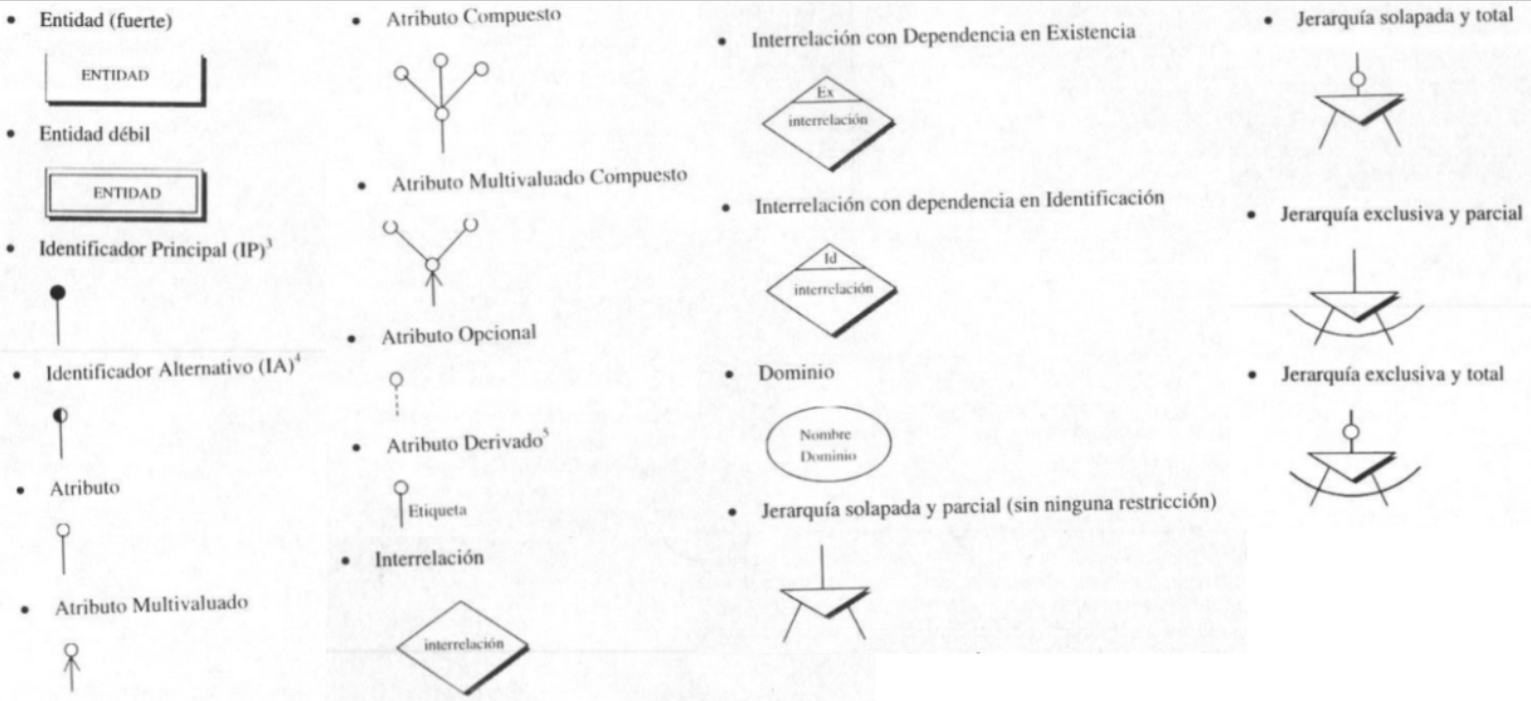
\includegraphics[width=\textwidth]{figures/notation}
    \caption{Conventions used for the graphical representation of the various constructs in the proposed E-R diagram problems.}
    \label{fig:notation}
\end{figure}

\subsection{How the problems are structured}

In order to facilitate the understanding of the proposed solutions to the modeling problems, each problem will be arbitrarily broken down into several steps.  In each step, a set of semantic assumptions will be studied that will give rise to an E-R sub-scheme.  In each step, elements will be added to the sub-scheme obtained in the previous step and so on until the study of all the semantic assumptions contemplated in the problem statement is completed.  We will assume that the statement constitutes a correct (and almost always complete) description of the Universe of Discourse.

An approach commonly used in the construction of E-R schemes is to first identify the entities, then the relationships, and finally the attributes of the entities and relationships.  In our case, all the elements (entities, attributes, relationships, cardinalities, etc.) will be identified for each set of semantic assumptions analyzed.  This may imply that some concepts are represented in the first steps with certain constructs and that later, in successive steps, the new semantic assumptions analyzed provide us with additional information that modifies some of the selected constructs.  For example, it could happen that a certain concept is represented in a first approximation as an attribute and that as the analysis of the assumptions of the statement progresses, it is discovered that it should be represented as an entity.

Sometimes other types of tools are also used that help us detect information that does not appear explicitly represented in the statement and that are very useful to inexperienced designers.  Thus, a proposal for a methodology for creating a conceptual scheme that takes these aspects into account would consist of the following steps:

\begin{enumerate}
    \item Study the statement that describes the Universe of Discourse and prepare two lists: one with the candidates to be entities and another with the possible relationships along with their correspondence type (1:1, 1:N, N:M).  In addition, those doubtful concepts that are not known how to represent (if as an entity or as a relationship) will be specified.
    \item Construct an Entity Matrix in which the rows and columns are names of entities and each cell may or may not contain names of relationships.  This matrix has the following aspect:

    \begin{verbatim}
        , E1 , E2 , E3 , EN
    E1  , I1 , I2 ,    , I3
    E2  ,    , I4 , I5 ,
    E3  ,    ,    , I6 ,
    EN  ,    ,    ,    , IN
    \end{verbatim}

    The entities are E1, E2,..., EN and the relationships are I1, I2, ..., IN.  As the matrix is symmetric, the cells that appear with a cross correspond to relationships that are already specified in the other half of the matrix.  The symbol in a cell indicates that there is no relationship between the two referenced entities.  In addition, the correspondence types of each relationship would have to be indicated.  For example, I1 could be a 1:N relationship.  It is important to note that this matrix does not collect relationships of a degree higher than two.  In the elaboration of this matrix, it is possible to detect relationships that do not appear explicitly represented in the statement and that, however, it might be interesting to include in the E-R scheme.  This type of relationship is generally detected by common sense, although it would always be necessary to validate them with the user.

    \item Using the entity matrix, a first E-R scheme is constructed with the entities, attributes, relationships, and their correspondence types.  The minimum and maximum cardinalities are added to this scheme.

    \item In this last step, the E-R scheme from the previous step is refined by studying the possible redundancies whenever there are cycles with semantically equivalent relationships.  This approach will be used in the first exercise of this topic.  Redundancy exists in an E-R scheme when the same semantics is collected in a duplicate manner, so that scheme could be represented while maintaining the same semantics with fewer elements.  In general, there can be redundancy when there are cycles in an E-R scheme (several entities joined by several semantically related relationships forming a cycle).  In this case, it would be necessary to check if by eliminating a relationship, the semantics represented in it can be obtained through the remaining relationships.  To do this, you have to study the cardinalities of the relationships in detail and do the check in both one direction and the other.  This process is described in De Miguel et al. (1999).  An example will be shown in the exercises of this chapter.
\end{enumerate}

\section{Problem 1:
Inhabitants and Municipalities
}

\subsection{Statement}

Suppose the following universe of discourse about municipalities, dwellings, and people.

Each person can only inhabit one dwelling and be registered in one municipality, but can own several dwellings.  We are also interested in knowing the people who depend on the Head of the Family (H.F.).  The semantic assumptions that are considered appropriate to justify all design decisions will be indicated.

\subsection{Discussion of the statement}

For the resolution of this exercise, the steps of a methodological guide for inexperienced designers will be followed:

\subsubsection*{Step 1: Elaborate the lists of candidate concepts to be entities and relationships and also indicate the concepts that are not known how to categorize.}

The lists obtained are:

\begin{itemize}
    \item \textbf{Entities}: MUNICIPALITY, DWELLING, PERSON
    \item \textbf{Relationships}: Inhabits between PERSON and DWELLING, Registered between PERSON and MUNICIPALITY, Property between PERSON and DWELLING
    \item \textbf{Uncertain}: HEAD OF FAMILY?
\end{itemize}

The previous entities and relationships are explicitly represented in the statement.  In principle, we do not know how to represent the concept Head of Family, since in reality it is also a Person.  We will leave the classification of this concept for the next step.

\subsubsection*{Step 2: Construct an Entities/Entities matrix to represent all the relationships along with their correspondence type.}

For this, we will analyze the semantic assumptions explicitly represented in the statement, as well as those that are implicit or common sense.

\textbf{A) Assumptions given in the statement:}

\begin{itemize}
    \item Each PERSON can only INHABIT one DWELLING (Inhabits relationship (1:?) between PERSON and DWELLING).
    \item Each PERSON can be the OWNER of more than one DWELLING (Property relationship (?:N) between PERSON and DWELLING).
    \item PERSONS depend on the head of the family (H.F. relationship (?:?) between PERSON and PERSON).
    \item A PERSON is registered in a single MUNICIPALITY (Registered relationship (1:N) between PERSON and MUNICIPALITY).
\end{itemize}

\textbf{B) Assumptions not given in the statement:}

\begin{itemize}
    \item Many PERSONS can INHABIT a DWELLING (logical assumption of the real world) -> Inhabits relationship (1:N) between PERSON and DWELLING.
    \item A DWELLING can be the PROPERTY of many PERSONS (legal assumption) -> Property relationship (M:N) between PERSON and DWELLING.
    \item A PERSON can only have one head of the family and a head of the family can be so for several PERSONS -> H.F. relationship (1:N) between PERSON and PERSON.
    \item A MUNICIPALITY can have many DWELLINGS and a DWELLING belongs to a single MUNICIPALITY -> Is\_In relationship (N:1) between MUNICIPALITY and DWELLING.
\end{itemize}

The resulting matrix is shown in figure 1.4.

\begin{figure}
    \centering
    % Placeholder for Figure 1.4
    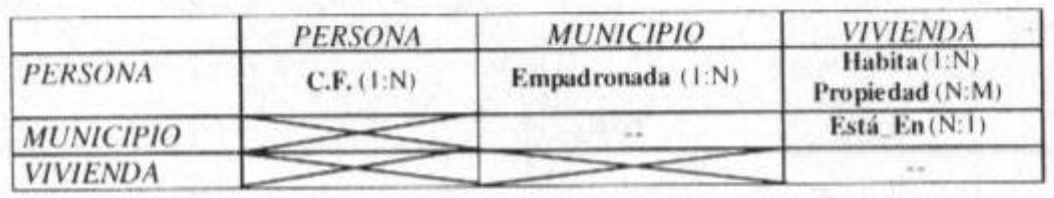
\includegraphics[width=0.6\textwidth]{figures/fig4}
    \caption{Entity/entity matrix. The table shows the relationships between PERSON, MUNICIPALITY, and DWELLING. PERSON to PERSON has a C.F. (1:N) relationship. PERSON to MUNICIPALITY has an Empadronada (N:1) relationship. PERSON to DWELLING has Habita (1:N) and Propiedad (N:M) relationships. MUNICIPALITY to DWELLING has an Está\_En (N:1) relationship.}
    \label{fig:fig1.4}
\end{figure}

\subsubsection*{Step 3: Obtain a preliminary version of the E-R scheme.}

Figure 1.5 shows a first version of the E-R Scheme corresponding to the mentioned assumptions.

\begin{figure}
    \centering
    % Placeholder for Figure 1.5
    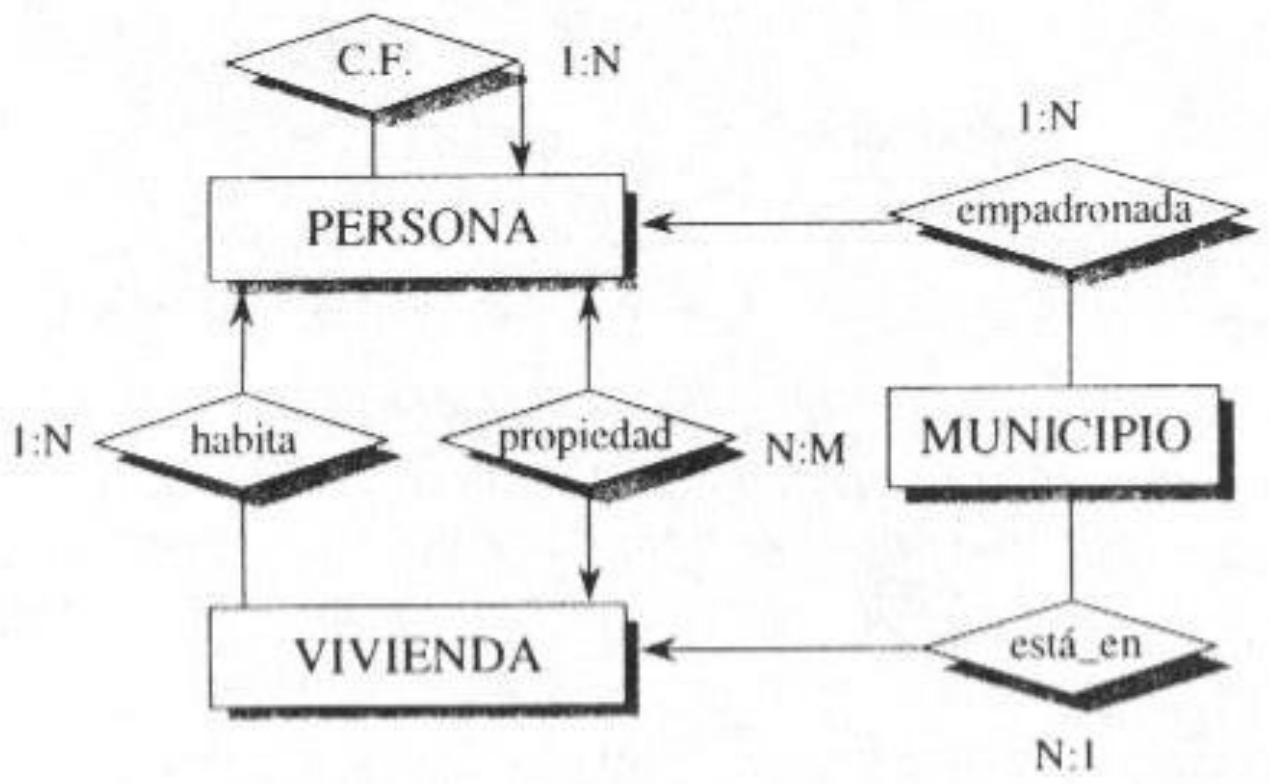
\includegraphics[width=0.8\textwidth]{figures/fig5}
    \caption{Preliminary version of the E-R scheme. This diagram shows the entities PERSON, DWELLING, and MUNICIPALITY with their relationships: C.F. (1:N) on PERSON, habita (1:N) and propiedad (N:M) between PERSON and DWELLING, empadronada (1:N) between PERSON and MUNICIPALITY, and está\_en (N:1) between DWELLING and MUNICIPALITY.}
    \label{fig:fig1.5}
\end{figure}

\subsubsection*{Step 4: Analysis of minimum cardinalities.}

So far, only the maximum cardinalities of the relationships have been studied.  Next, the minimum cardinalities will be studied.

\begin{itemize}
    \item \textbf{C.F. Relationship}: A PERSON must have at least one PERSON who is the Head of the Family, and a PERSON who is the Head of the Family may not have anyone in their charge.
    \item \textbf{Inhabits Relationship}: A PERSON inhabits at least one DWELLING and in a DWELLING no PERSON may inhabit it.
    \item \textbf{Property Relationship}: A PERSON may not own any DWELLING and a DWELLING may not be the property of any PERSON (a dwelling could be owned by a company, for example).
    \item \textbf{Registered Relationship}: A PERSON is registered in at least one MUNICIPALITY (and at most also) and in a MUNICIPALITY at least one PERSON is registered.
    \item \textbf{Is\_In Relationship}: A DWELLING is in a single MUNICIPALITY and in a MUNICIPALITY there is at least one DWELLING.
\end{itemize}

Figure 1.6 shows the E-R diagram with the maximum and minimum cardinalities.

\begin{figure}
    \centering
    % Placeholder for Figure 1.6
    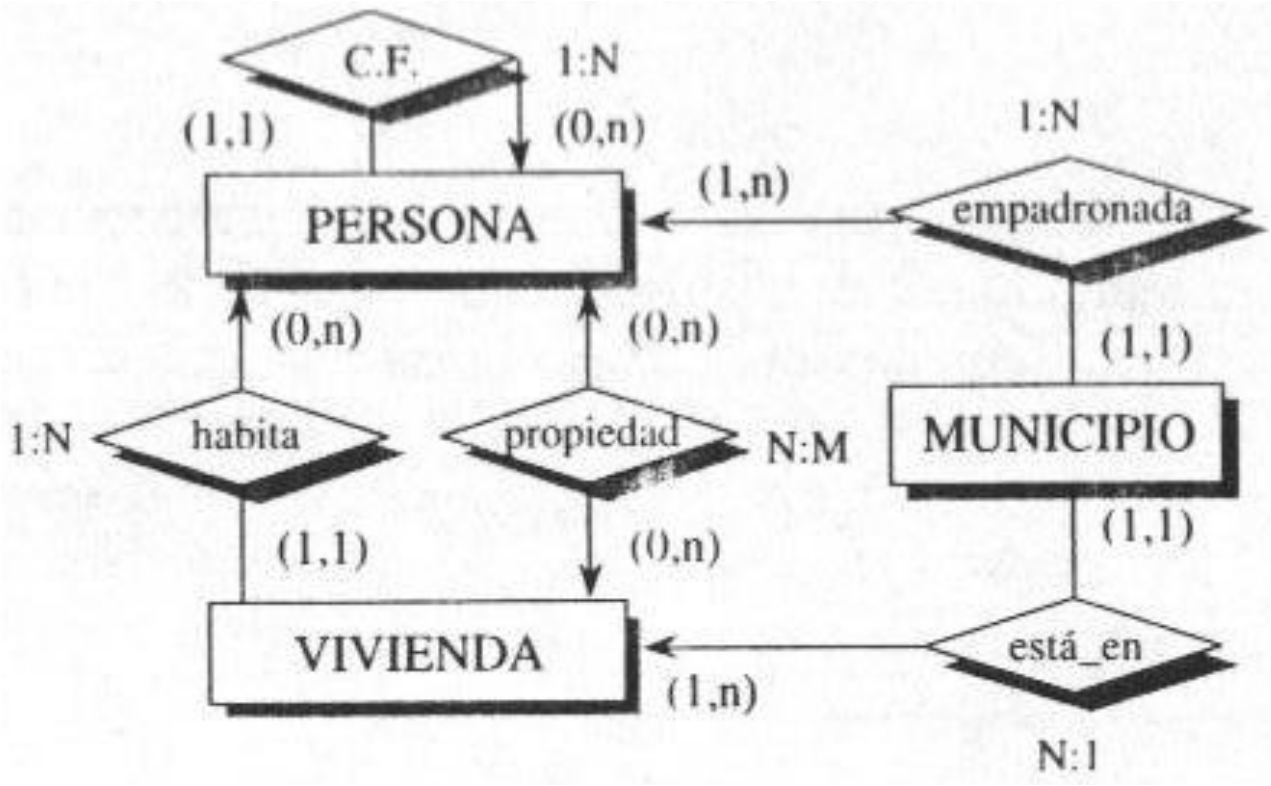
\includegraphics[width=0.8\textwidth]{figures/fig6}
    \caption{E-R scheme with cardinality constraints. This is a more detailed version of the previous E-R diagram, adding minimum and maximum cardinalities to the relationships, such as (1,1), (0,n), etc.}
    \label{fig:fig1.6}
\end{figure}

\subsubsection*{Step 5: Analysis of redundancies.}

As there are two cycles in the E-R scheme, it is necessary to study if there is any redundant relationship, that is, if there is any relationship whose semantics can be obtained from the other relationships.

The first cycle is made up of the Property, Is\_In, and Registered relationships.  The first condition to know if we have a cycle in which there is a relationship likely to be redundant is that the three relationships are semantically related.  In this case, the Property relationship is not semantically equivalent to Is\_In and Registered, since owning or not owning a dwelling does not influence whether the person resides in the municipality where the dwelling is located.

The second cycle is made up of the Inhabits, Is\_In, and Registered relationships.  In this case, the three relationships are semantically related.  Let's see if any of these relationships are redundant:

\begin{itemize}
    \item \textbf{Inhabits Relationship}: If we try to eliminate the Inhabits relationship, it must be possible to obtain its semantics from Is\_In and Registered; thus, if we want to obtain the people who inhabit a certain dwelling, from Is\_In we obtain the municipality in which the dwelling is located and with the Registered relationship we obtain the people who inhabit that municipality, but we do not know the people who inhabit the dwelling but those who inhabit all the dwellings of the municipality.  Therefore, the Inhabits relationship cannot be eliminated.  We assume that people live in the municipalities where they are registered.

    \item \textbf{Is\_In Relationship}: If we try to suppress the Is\_In relationship, it must be possible to obtain its semantics from the Inhabits and Registered relationships.  To know the dwellings that are in a certain municipality, from Registered we obtain all the people registered in that municipality and through the Inhabits relationship we obtain the dwellings in which those people live (since a person must necessarily live in a dwelling); in this way, we will know the dwellings of that municipality.  In the other direction of the Is\_In relationship, to know in which municipality a certain dwelling is, from Inhabits we obtain the people who live in it; however, it may happen that in a certain dwelling no one lives (minimum cardinality 0), so we cannot reach the Registered relationship between person and municipality.  Thus, the Is\_In relationship is not redundant.

    \item \textbf{Registered Relationship}: If we eliminate the Registered relationship, it should be possible to obtain its semantics from Inhabits and Is\_In.  To know the municipality in which a person is registered, through Inhabits we obtain the dwelling in which that person lives and with the Is\_In relationship we obtain the municipality in which the dwelling is located; Therefore, we know the municipality in which that person is registered.  In the other direction of the Registered relationship, it must be possible to know the people registered in a certain municipality: through the Is\_In relationship we know the dwellings of that municipality and from Inhabits we know all the people who live in those dwellings, thus knowing all the people registered in the municipality.  Consequently, the Registered relationship can be eliminated from the E-R scheme without losing semantics.
\end{itemize}

The definitive E-R scheme is shown in figure 1.7.

\begin{figure}
    \centering
    % Placeholder for Figure 1.7
    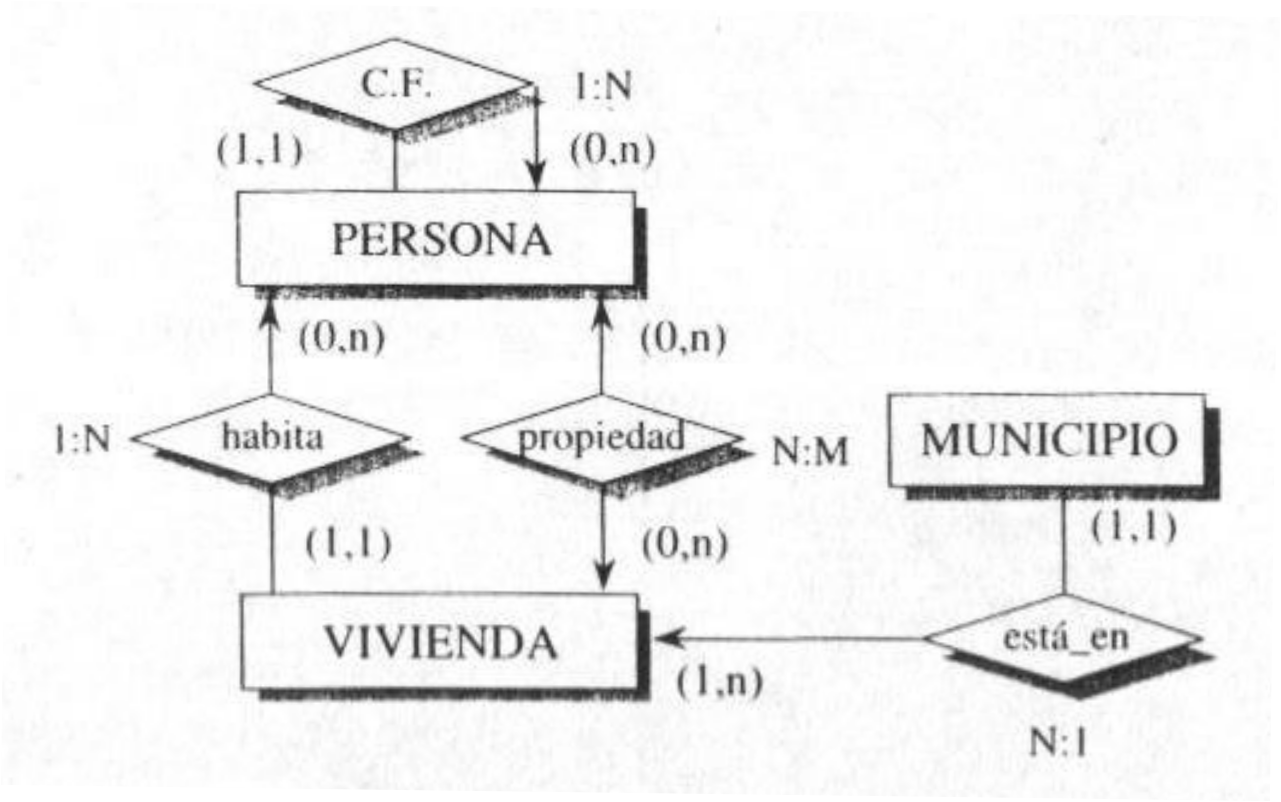
\includegraphics[width=0.8\textwidth]{figures/fig7}
    \caption{E-R scheme without redundancies. The final diagram after removing the redundant 'empadronada' relationship. It shows PERSON, DWELLING, and MUNICIPALITY entities with the remaining relationships: C.F., habita, propiedad, and está\_en, along with their cardinalities.}
    \label{fig:fig1.7}
\end{figure}

\subsection*{
Supplementary Semantic Assumptions and Unreflected Semantics
}

All the semantics of the problem has been reflected, and it has not been necessary to make additional assumptions.

\section{Problem 2: Training Courses}

\subsection{Statement}

The training department of a company wants to build a database to plan and manage the training of its employees.

The company organizes internal training courses for which it is desired to know the course code, the name, a description, the number of hours of duration, and the cost of the course.

A course may have as a prerequisite to have previously completed another course(s), and, in turn, the completion of a course may be a prerequisite for others.  A course that is a prerequisite for another can be so on a mandatory or only recommended basis.

The same course has different editions, that is, it is taught in different places, dates, and with different schedules (intensive, morning, or afternoon).  On the same start date, only one edition of a course can be taught.

The courses are taught by personnel from the company itself.

Of the employees, it is desired to store their employee code, name and surname, address, telephone, NIF (Tax Identification Number), date of birth, nationality, sex, signature, and salary, as well as whether or not they are qualified to teach courses.

The same employee can be a teacher in one edition of a course and a student in another edition, but can never be both at the same time (in the same edition of a course, he either teaches it or receives it).

\end{document}
